%
%
%

\begin{frame}[t,allowframebreaks]{Increasing neural network size - }

    % Intro

    % Number of connections in various artificial neural nets as a function of time
    % and comparison with biological brains

    The human brain has $\sim$100 billion neurons and $\sim$100 trillion synapses!

    \begin{center}
        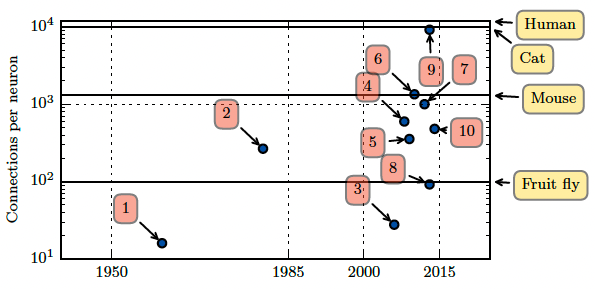
\includegraphics[width=0.95\textwidth]
          {./images/dl_intro/nnet_size_connections_vs_time_01.png}\\
        {\scriptsize \color{col:attribution} 
        Reproduced from p.22 of \cite{Goodfellow:2017DL}}\\
    \end{center}

    \framebreak

    % Number of neurons in various artificial neural nets as a function of time
    % and comparison with biological brains

    \begin{center}
        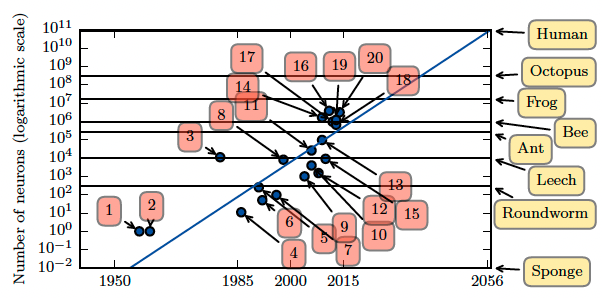
\includegraphics[width=0.95\textwidth]
           {./images/dl_intro/nnet_size_neurons_vs_time_01.png}\\
        {\scriptsize \color{col:attribution} 
        Reproduced from p.23 of \cite{Goodfellow:2017DL}}\\
    \end{center}
       {\tiny
       1. Perceptron (1958) \cite{Rosenblatt:1958p},
       2. Adaptive linear element (1960) \cite{Widrow:1960as},
       3. Neocognitron (1980) \cite{Fukushima:1980nc},
       4. Early back-propagation network (1986) \cite{Rumelhart:1986erp},
       5. Recurrent neural network for speech recognition (1991) \cite{Robinson:1991rerp},
       6. Multilayer perceptron for speech recognition (1991) \cite{Bengio:1991pma},
       7. Mean field sigmoid belief network (1996) \cite{Saul:1996mf},
       8. LeNet-5 (1998) \cite{LeCun:1998ln5},

       9. Echo state network (2004) (Jaeger and Haas, 2004)
       10. Deep belief network (2006) (Hinton et al., 2006)
       11. GPU-accelerated convolutional network (2006) (Chellapilla et al., 2006)
       12. Deep Boltzmann machine (2009) (Salakhutdinov and Hinton, 2009a)
       13. GPU-accelerated deep belief network (2009) (Raina et al., 2009)
       14. Unsupervised convolutional network (2009) (Jarrett et al., 2009)
       15. GPU-accelerated multilayer perceptron (2010) (Ciresan et al., 2010)
       16. OMP-1 network (2011) (Coates and Ng, 2011)
       
       17. Distributed autoencoder (2012) \cite{Le:2012daut}
       18. Multi-GPU convolutional network (2012) \cite{Krizhevsky:2012img},
       19. COTS HPC unsupervised convolutional network (2013) \cite{Coates:2013cots},       
       20. GoogLeNet (2014) \cite{Szegedy:2014gnet}\\
       }

    \framebreak

    % Information from recent well-known artificial neural networks

    \begin{itemize}
        \item GPT-2 had 1.5 billion parameters and around 50 billion neurons
        \item GPT-3 is estimated to have around 60-80 billion neurons
        \item GPT-4 is estimated to have around 60-80 billion neurons
    \end{itemize}

\end{frame}
